% Paleta pastel alternativa (nuevos matices)
\definecolor{FixationColor}{HTML}{BFD8B8} % sage
\definecolor{MotorColor}{HTML}{F6C28B}    % peach/sand
\definecolor{RestColor}{HTML}{A7C5EB}     % powder blue
\definecolor{InterColor}{HTML}{EDE6F2}    % mist lavender-gray
\definecolor{CueColor}{HTML}{B5EAEA}      % mint

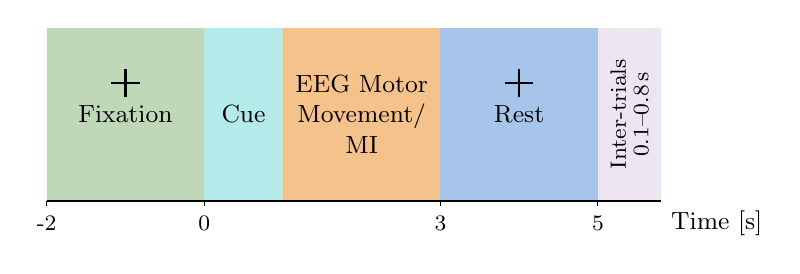
\begin{tikzpicture}
  % ===== Parámetros =====
  \def\boxheight{2.2}
  \def\startFix{-2}
  \def\endFix{0}
  \def\endCue{1}      % Duración del cue (0–1 s). Cambia a 0.8 si lo quieres más corto
  \def\endMI{3}
  \def\endRest{5}
  \def\endInter{5.8}

  \def\plusLen{0.18}  % Tamaño de la cruz (+); baja este valor para hacerla más pequeña
  \def\showPlusInRest{1} % 1=mostrar cruz en Rest, 0=ocultar

  % ===== Bloques =====
  \fill[FixationColor] (\startFix,0) rectangle (\endFix,\boxheight);
  % MI SIN cruce con cue: inicia en 1 s
  \fill[MotorColor]    (\endCue,0)   rectangle (\endMI,\boxheight);
  \fill[RestColor]     (\endMI,0)    rectangle (\endRest,\boxheight);
  \fill[InterColor]    (\endRest,0)  rectangle (\endInter,\boxheight);
  % Cue como bloque vertical (0–1 s)
  \fill[CueColor]      (\endFix,0)   rectangle (\endCue,\boxheight);

  % ===== Etiquetas =====
  \node[font=\small]              at ({(\startFix+\endFix)/2},{0.5*\boxheight}) {Fixation};
  \node[font=\small,align=center] at ({(\endCue+\endMI)/2},{0.5*\boxheight}) {EEG Motor\\Movement/\\MI};
  \node[font=\small]              at ({(\endMI+\endRest)/2},{0.5*\boxheight}) {Rest};
  \node[font=\footnotesize,rotate=90]
       at ({(\endRest+\endInter)/2},{0.5*\boxheight}) {\shortstack{Inter-trials\\0.1--0.8\,s}};
  \node[font=\small]              at ({(\endFix+\endCue)/2},{0.5*\boxheight}) {Cue};

  % ===== Cruces (+) =====
  % Fixation
  \pgfmathsetmacro{\xfix}{(\startFix+\endFix)/2}
  \pgfmathsetmacro{\yfix}{0.68*\boxheight}
  \draw[line width=0.8pt] (\xfix,\yfix-\plusLen) -- (\xfix,\yfix+\plusLen);
  \draw[line width=0.8pt] (\xfix-\plusLen,\yfix) -- (\xfix+\plusLen,\yfix);

  % Rest (opcional)
  \ifnum\showPlusInRest=1
    \pgfmathsetmacro{\xrest}{(\endMI+\endRest)/2}
    \pgfmathsetmacro{\yrest}{0.68*\boxheight}
    \draw[line width=0.8pt] (\xrest,\yrest-\plusLen) -- (\xrest,\yrest+\plusLen);
    \draw[line width=0.8pt] (\xrest-\plusLen,\yrest) -- (\xrest+\plusLen,\yrest);
  \fi

  % ===== Eje X =====
  \draw[thick] (\startFix,0) -- (\endInter,0) node[below right,font=\small] {Time [s]};
  \foreach \x/\lbl in {\startFix/-2, 0/0, \endMI/3, \endRest/5}{
    \draw (\x,0) -- ++(0,-2pt) node[below,font=\footnotesize] {\lbl};
  }

\end{tikzpicture}